%!TEX root = ../dokumentation.tex

\chapter{Method}

\section{Catalogue of Criteria}

For measuring the success of this project afterwards some criteria need to be defined of what should be achieved during this project.

The longterm goal for the car sharing project is to move away from a local setup to a deployment on a cluster with all its components and dependencies.

The first step for that is to outsource the Kafka client from a local setup to a Cloud service. For that the IBM Cloud Message Hub service can be used. This also enables the possibility to send request not only from the local device, on which the car sharing app itself is running, but also from other applications like a mobile device, which is a necessary requirement for a real use of the car sharing app. Because currently there is no clean way of testing the Kafka client also a web application for testing purposes of the Kafka client should be created. This app should be able to produce messages as well as consuming them and printing them on its UI, so that it can be checked if the production of messages is successfull and, that they can be consumed afterwards.

After that the DummyScheduler should be deployed on the Cluster. This requires to create a container of the car sharing app. Because the DummyScheduler does not use the cplex engine or any other third party service those dont need to be included to the Docker container.

Because the cluster is an internal Research Cluster there are some differences to "normal" Kubernetes cluster. This causes some additional security stepts to be made for deploying apps on it. These additional stepts should be figured out and documented, so that it can be done with other apps without the need of additional research in the future.

If the DummyScheduler is running on the cluster, all its functionalities are working and the Kafka client is outsourced to the IBM Cloud Message Hub, the project can be considered as successful.

If the deployment of the car sharing app, for example with the real scheduler and its requirements, can get continued beyond that, the project can be considered as overachieved.

\section{Local setup of car sharing app}

For a better understanding of how the car sharing app is working and how the infrastructure for the communication with its underlying services is build up, first the   actual state with local setup of all the single components will be described and explained.

For enabling all functions of the car sharing app, three services need to be setup beforehand. Those are Apache Kafka, OSRM and Mongo Database. First it will be explained how those services can be setup and what they are needed for.

Apache Kafka needs to run on top of a Apache Zookeeper instance. Zookeeper is a a centralized service for maintaining naming and configuration data and providing synchronization within distributed systems. For Kafka it keeps track of status of the cluster nodes as well as its topics, partitions etc. \textsuperscript{cmp.\cite{38}}

%https://www.cloudkarafka.com/blog/2018-07-04-cloudkarafka_what_is_zookeeper.html

The Kafka service as well as the Zookeeper are running inside of two separated docker containers. The kafka container listens on port 9092 for predefined topics. In the case of the car sharing app those topics are ``book'' and ``confirm''. A Kafka client inside the car sharing app provides a producer as well as a consumer. The consumer listens on new messages for the ``book'' topic. This way the app is able to receive booking request for the car sharing service, so that customer can request a ride. This ride needs to be confirmed then, which the producer is for. It can produce messages to the ``confirm'' topic, so that the consumer can be informed about the approval of his ride request and additional information like estimated arriving time or car identification.

For testing the Kafka client within the in this essay described work a test web application was developed. This enables entering a topic, a key and a value and producing a message. This message is then produced by a provided producer.  Also the test apps provides two consumers - one listening on the ``book'' topic, another one listening on the ``confirm'' topic. This way it can be controlled, if all produced messages of this topic are successfully produced to the Kafka service and if they can be consumed by the consumer. All consumed messages are shown directly on the Web UI, which allows dynamic changes via the Python SocketIO library.

The scheduler uses this for listening to requests, calculating the best fitting car and its route and confirming the ride after all calculations have been made. In the current state of the project there are two different Schedulers - first the ``real'' scheduler, which is yet only implemented for a simulation, so that it gets its request from a predefined file instead of a Kafka consumer. The other scheduler is a ``dummy'' scheduler, which is used for a demonstration with a real car, for which no complicated scheduling is necessary, because it is only one car. This ``dummy'' scheduler uses kafka for consuming requests and confirms them directly afterwards with an equal message for the ``confirm'' topic.

%check if no kafka client for real scheduler

The second underlying service for the car sharing app is OSRM. As described in chapter INSERT OSRM is for calculating the shortest paths in road networks. For this a map is needed in \acs{PBF} (\acl{PBF}) format. This map then needs to be extracted with a car profile, which determines which routes or streets can be used for this kind of vehicle and which cannot (private road, barriers etc.). This also converts the map into an osrm file. Next this needs to be partitioned into cells and last these cells have to get customized by calculating its routing weights. This OSRM container is also setup within a docker container listening to port 3000 of the localhost for requests for calculating routes on the given map. For running the necessary steps for preparing the map inside the docker container there is a preprocessing shell script prepared, looking like this:

%https://github.com/Project-OSRM/osrm-backend/wiki/Running-OSRM

\begin{lstlisting}
rm -rf "$(pwd)"/data/*.osrm
rm -rf "$(pwd)"/data/*.osrm.*

docker run -t --rm -v "$(pwd)"/data:/data osrm/osrm-backend osrm-extract -p /opt/car.lua /data/new-york.osm.pbf
docker run -t --rm -v "$(pwd)"/data:/data osrm/osrm-backend osrm-partition /data/new-york.osrm
docker run -t --rm -v "$(pwd)"/data:/data osrm/osrm-backend osrm-customize /data/new-york.osrm
\end{lstlisting}

The map data are not stored inside the docker container itself but on the local system. This data is then mounted to the docker container, so that it can access it without the need of storing it inside, which keeps the docker container more light weighted.

The third service is a Mongo Database, on which all vehicles, customers, routes and the history are stored. Through this a demo UI can access all necessary informations to represent the vehicles, customers and its calculated routes. This database can be created by a mongo seed, in which all necessary informations are stored in a compact format, so that the database can easily be restored. 

The MongoDB is also running inside a Docker container. The needed seed data are mounted to the Docker container, so that it can access these data stored on the local machine from within the container. Also the created database is created in a local directory which is then mounted to the Docker container. The database is restored by running a mongo-seed shell script looking like this, which first drops the existing table and then recreate a new one by the stored seed:

%check tables

\begin{lstlisting}
mongo db_rs --eval "db.dropDatabase()"
mongorestore --db db_rs --dir /tmp/seed/data
\end{lstlisting}

This script is executed within the docker container by running this command:

\begin{lstlisting}
docker exec -it cs-mongo sh -c "chmod 700 /tmp/seed/mongo-seed.sh && /tmp/seed/mongo-seed.sh"
\end{lstlisting}

With all those services running now the car sharing app itself can be started. For the DummyScheduler only the Kafka service is needed. For the simulation all of those services are necessary but the Kafka service. How the communication works can be withdrawn by the following figure, which uses the simulation as example application.

\begin{figure}[h]
\centering
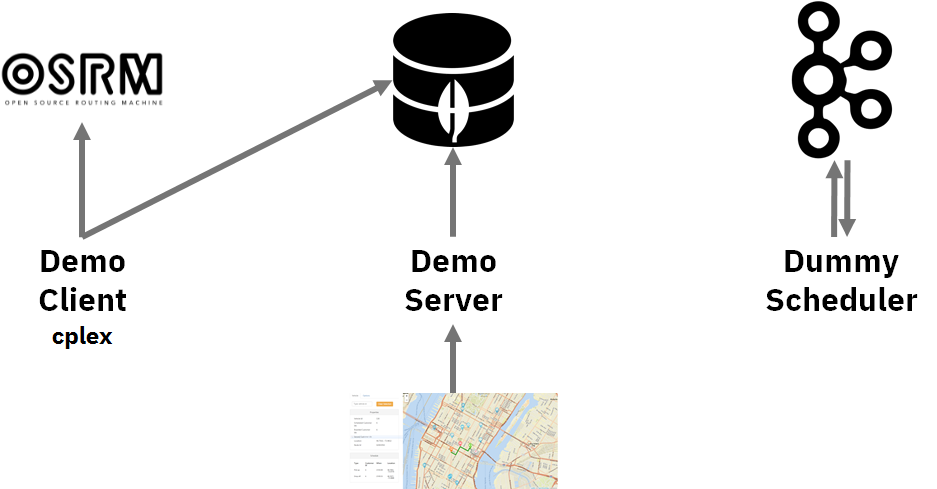
\includegraphics[width=\textwidth/5*4]{images/simulation_communication.png}

\textsuperscript{Figure 3.2.1 Simulation communication with services}\\
\end{figure}

The car sharing simulation needs two components running - first the demo client and second the demo server. The client runs through predefined requests stored in a json file. Those requests are processed by the scheduler, which calculates the route with OSRM. For optimizing the route the cplex engine is used. After completing the calculations the results are written to the mongo database. The demo server consists out of an API, which can be accesses for requesting the current state of all vehicles, customers and calculated routes. For that it connects to the Mongo database and returns the requested data. This is how the simulation can be visualized on a demo UI, which sends requests to the server and represents the current state on a graphical map.

%cplex?

\section{Outsourcing Kafka client to IBM Cloud message hub}

The locally running Kafka service has two disadvantages: The first one is, that it needs to be setup along with Zookeeper every time when running the app. For deploying the car sharing app within a cluster on the cloud the Kafka client as well as an underlying Zookeeper would also have to get deployed on it to guarantee the functionality of the car sharing app.

The second problem is, that a local Kafka client can only be accessed from local side. This means, that no messages can be produced to the Kafka client from outside the host, which prevents the car sharing app from receiving customer requests from the outside, for example an app with which the customers can order a ride.

These problems can be solved by outsourcing the 	Kafka client to a Cloud service like the IBM Cloud Message Hub. This service contains a fully managed, highly scalable and high performing Kafka platform. In this chapter it will be described how the configurations of the car sharing kafka client has to be changed, so that it can connect to the IBM Cloud Message Hub.

%https://www.ibm.com/cloud/message-hub???

Currently there are several configurations made for the local Kafka client. These configurations can be found in the following figure

\begin{lstlisting}
    KAFKA_BROKER = "localhost:9092"
    KAFKA_BOOKING_TOPIC = "book"
    KAFKA_CONFIRMATION_TOPIC = "confirm"
    KAFKA_TOPICS = [KAFKA_BOOKING_TOPIC, KAFKA_CONFIRMATION_TOPIC]
    KAFKA_GROUP = "group1"
    KAFKA_TOPIC_CONFIG = {"auto.offset.reset": "smallest"}
    KAFKA_CONSUMER_SESSION_TIMEOUT_MS = 30000
\end{lstlisting}

First the broker is set to the localhost with port 9092 before the booking and confirmation topics names are set. After that there are just some general settings to be made for the Kafka client like session timeout. They will stay the same with the Message Hub configurations. For this there are some additional settings to add for enabling access to the Kafka Client running on the IBM Cloud service. The new configurations are listed below.

\begin{lstlisting}
    KAFKA_BROKER = os.getenv("BOOTSTRAP_SERVERS")
    KAFKA_BOOKING_TOPIC = "book"
    KAFKA_CONFIRMATION_TOPIC = "confirm"
    KAFKA_TOPICS = [KAFKA_BOOKING_TOPIC, KAFKA_CONFIRMATION_TOPIC]
    KAFKA_GROUP = "group1"
    KAFKA_TOPIC_CONFIG = {"auto.offset.reset": "smallest"}
    KAFKA_CONSUMER_SESSION_TIMEOUT_MS = 30000
    KAFKA_SECURITY_PROTOCOL = 'SASL_SSL'
    KAFKA_SSL_CA_LOCATION = '/etc/ssl/certs'
    KAFKA_SASL_MECHANISMUS = 'PLAIN'
    KAFKA_SASL_USERNAME = 'token'
    KAFKA_SASL_PASSWORD = os.getenv("API_KEY")
    KAFKA_API_VERSION_REQUEST = True
    KAFKA_BROKER_VERSION_FALLBACK = '0.10.2.1'
    KAFKA_LOG_CONNECTION_CLOSE = False
    KAFKA_CLIENT_ID= 'client1'
    KAFKA_GROUP_ID = "group1"
\end{lstlisting}

First there are the same configurations to be made as for the local client. Only the broker needs to be changed. In this case it takes the broker out of an environment file, in which the url of the broker is defined. Addtionally there are settings for a secure access to the broker, like used security protocol or ssl location. For the identification an API token is used. That's why the username is set to ``token''. The password has to equal the API key in this case, which is also read from the environment file. Both - the API key as well as the broker - can be found on the IBM Cloud Message Hub dashboard. Last there are some more configurations for the API access, version and logging to be made.

These configurations are added as additional configuration mode called ``MessageHubConfig'' in the configuration file. To use these configurations the used mode has to be changed to the newly added ``MessageHubConfig''.

When configuring the Kafka client later in the app sequence it will access this configurations to set it up. Because there are some new configurations and not only existing ones with different values, these have also to be added to the setup of the Kafka client. There a JSON is created like below:

\begin{lstlisting}
        'bootstrap.servers': config.KAFKA_BROKER,
        'session.timeout.ms': config.KAFKA_CONSUMER_SESSION_TIMEOUT_MS,
        'default.topic.config': config.KAFKA_TOPIC_CONFIG,
        'batch.timeout_s': config.BOOKING_REQUEST_PROCESSOR_BATCH_TIMEOUT_S,
        'batch.topics': [config.KAFKA_BOOKING_TOPIC],
        'batch.job.trigger.default.interval_s': config.BOOKING_REQUEST_PROCESSOR_TIME_WINDOW_S,
        'batch.executor.default.pool': 1,
        'batch.job.max_instances': 1,
        'security.protocol': config.KAFKA_SECURITY_PROTOCOL,
        'ssl.ca.location': config.KAFKA_SSL_CA_LOCATION,
        'sasl.mechanisms': config.KAFKA_SASL_MECHANISMUS,
        'sasl.username': config.KAFKA_SASL_USERNAME,
        'sasl.password': config.KAFKA_SASL_PASSWORD,
        'api.version.request': config.KAFKA_API_VERSION_REQUEST,
        'broker.version.fallback': config.KAFKA_BROKER_VERSION_FALLBACK,
        'log.connection.close': config.KAFKA_LOG_CONNECTION_CLOSE,
        'client.id': config.KAFKA_CLIENT_ID,
        'group.id': config.KAFKA_GROUP_ID,
\end{lstlisting}

This takes all the configurations made in the CONFIGURATION file and add these to a JSON, which is used for the initialization of the Kafka producer as well as its consumer. After adding these configurations the Kafka client is successfully setup for accessing the IBM Cloud Message Hub Kafka service.

\section{Dockerizing car sharing app and underlying technologies}

For deploying the car sharing app and all its underlying technologies on a Kubernetes cluster it needs to be dockerized beforehand. This means, that the application needs to be packed in a container, in which only the app itself and a very light weighted \acs{OS} (\acl{OS}) with only necessary installations are running. This is made possible by Docker.

In every Docker container only one application can be running at the same time. That's why for every application needed for the car sharing app, an own Docker container is needed. That means all in all three Docker containers are needed - one for the MongoDB, one for OSRM and one for the car sharing app itself. 
To build a Docker container it is necessary to create a Dockerfile. This Dockerfile is usually based on one basic image, like a very light weighted Ubuntu OS, and then every necessary step to be taken before the app can be executed. This includes copying necessary data, setting environment variables, installing necessary compilers and libraries etc. 

For Mongo and OSRM there are already prebuilt Docker containers exisiting. They need to be extended by the necessary data for the car sharing app and the operations needed to be executed on these data. In case of OSRM such a Dockerfile looks like this:

\begin{lstlisting}
FROM osrm/osrm-backend

COPY ./osrm/data/new-york.osm.pbf /opt
RUN osrm-extract -p /opt/car.lua /opt/new-york.osm.pbf
RUN osrm-partition /opt/new-york.osrm
RUN osrm-customize /opt/new-york.osrm

CMD ["osrm-routed", "--algorithm", "mld", "/opt/new-york.osrm"]
\end{lstlisting}

First the base image is defined with the ``FROM'' command. Then the map is copied and the necessary preprocessing commands described in chapter 3.2 are executed. Last the osrm service is started with the prepared map in the ``CMD'' statement.

Extending the Mongo Docker container works similarly:

\begin{lstlisting}
FROM mongo:3.4
MAINTAINER Pascal Schroeder <pascal.schroeder@de.ibm.com>

COPY ./mongo/seed /tmp/seed

ENV MONGO_DATA_DIR=/data/db
ENV MONGO_LOG_DIR=/dev/null

RUN chmod 700 /tmp/seed/mongo-seed.sh

CMD mongod --fork --logpath /var/log/mongodb.log; \
    ./tmp/seed/mongo-seed.sh; \
    mongo db_rs --eval 'db.network.createIndex( { "lat_lon" : "2d" } );'; \
    mongod --shutdown; \
    docker-entrypoint.sh mongod
\end{lstlisting}

First the base image is declared. Then the seed folder is copied into the docker container, so that it can use the seed for restoring the database afterwards. Then a few necessary environment variables are set before the ``mongo-seed.sh'' file is set to executable. When starting the mongo database it first runs the ``mongo-seed.sh'' script for restoring the database and creates the necessary index before restarting the mongo database.

Last the car sharing app itself needs to be dockerized. For that there is no prebuilt docker container, so this image is based on a light weighted ubuntu version and installs every requirement itself. This Dockerfile looks like this:

\begin{lstlisting}
FROM ubuntu:latest
MAINTAINER Pascal Schroeder <pascal.schroeder@de.ibm.com>

RUN apt-get update 
RUN apt-get install -y locales
RUN apt-get dist-upgrade -y
RUN apt-get update

ENV PYTHONPATH=/drl-car-sharing
ENV TZ=Europe/Dublin

RUN mkdir -p /drl-car-sharing
WORKDIR /drl-car-sharing
COPY . .

RUN apt-get install python3 python3-pip -y

RUN cd ./cplex/x86-64_linux && python3 setup.py build && python3 setup.py install

RUN pip3 install -r requirements.txt

WORKDIR /drl-car-sharing/drl_car_sharing/srv
CMD ["python3", "launch-query-proc.py"]
\end{lstlisting}

First the \acs{apt} (\acl{apt}) get updated and the locales package gets installed as well as the distribution gets upgraded. Then some environment variables for the pythonpath and the timezone are set before the work directory is created and set. Then all the project files are copied into the docker container except for the not-required files defined in the ``.dockerignore'' file.

After that python3 gets installed as well as the python package manager \acs{pip} (\acl{pip}).  Then it installs the requirements of this project defined in the ``requirements.txt''. 

Last the directory is changed and the file to be executed for starting the app is defined. In this case it is the file for the DummyScheduler. For starting another file, for example the simulation, it is necessary to create a new Dockerfile based on this image, which changes the file to be executed in the end. This looks like following code snippet:

\begin{lstlisting}
FROM registry.eu-de.bluemix.net/drlautopilot/drl-car-sharing

ENV PYTHONUNBUFFERED = 0

WORKDIR ../demo
CMD ["python3", "-u", "start_demo_cli.py"]
\end{lstlisting}

To build these Dockerfiles the docker build command has to be run. This command can be found below

\begin{lstlisting}
docker build -t <tag-of-docker-image> -f <name-of-dockerfile> <path-to-dockerfile>
\end{lstlisting}

The <tag-of-docker-image> is needed for the identification. Also with the tag it can be defined to which registry the image will be pushed. This is explained in more detail in chapter 3.5. The <name-of-dockerfile> is only needed when the Dockerfile is not called Dockerfile. Otherwise this parameter can be removed of this command. The <path-to-dockerfile> parameter is necessary and defines the relative path to the Dockefile. 

After the Docker images are all built they can be pushed to a container registry. How this works and how they can be deployed on a cluster afterwards is described in chapter 3.5.


\section{Deploying and exposing docker container on cluster}

Before deploying a Docker container on a Kubernetes cluster, the containers need to be pushed to a container registry, from where the cluster can access and pull the image. One possibility is the open platform DockerHub. It is the largest community for container images and for example the base images for mongo and OSRM are already stored on it. The disadvantage is, that they the containers are stored on public servers and even, if they can be set to private containers, unpermitted access to the data can not be guaranteed. 

That's why for confidential data private container registries are usually preferred. In case of the car sharing project this is the IBM Cloud container registry. To push a container to this registry it needs to be correctly tagged. For that the tag needs to start with \textit{registry.<region>.bluemix.net/<namespace>}. The \textit{<region>} placeholder has to be replaced with the location of the used container registry, for example ``eu-de''. In those container registry services of IBM cloud there can be created different namespaces. For defining them in the tag the \textit{<namespace>} placeholder has to be replaced with the chosen namespace. The docker image with id \textit{<image-id>} can be tagged with

\begin{lstlisting}
docker tag <image-id> registry.eu-de.bluemix.net/<your-namespace>/<name-of-image>
\end{lstlisting}

Before pushing the container the user has to be logged in to IBM Cloud \acs{CLI} (\acl{CLI}) and an account, a region and a Cloud space has to be chosen. After that it can be pushed with the docker push command and the newly generated tag:

\begin{lstlisting}
docker push <image-id> registry.eu-de.bluemix.net/<your-namespace>/<name-of-image>
\end{lstlisting}

Now the docker image is ready to get deployed on the Kubernetes cluster. This has to be repeated for every docker container to be deployed. This means in case of the car sharing project this has to be done for the extended mongo and osrm docker container as well as the car sharing containers for the simulation as well as the scheduler component itself. For deploying those containers to the cluster a deployment.yaml file is needed. Before that a secret for pulling the image from the cloud registry needs to be created beforehand. When a secret is created it needs to be defined in the deployment.yaml along with other properties. All in all this file has to look like below:

\begin{lstlisting}
apiVersion: extensions/v1beta1
kind: Deployment
metadata:
  name: <name-of-deployment>
spec:
  selector:
    matchLabels:
      app: <name-of-deployment>
  replicas: 1
  template:
    metadata:
      labels:
        app: <name-of-deployment>
    spec:
      containers:
      - name: <name-of-container>
        image: <tag-of-container>
        resources:
          requests:
            cpu: <requestes-cpu-power>
            memory: <requested-memory>
          limits:
            cpu: <max-cpu-power>
            memory: <max-memory>
      imagePullSecrets:
      - name: <name-of-secret>
\end{lstlisting}

In this example deployment.yaml several properties needs to be changed. First, the <name-of-deployment> placeholders have to be set to the name, which the deployment itself will get. The <tag-of-container> placeholder has to equal the tag with which the container was tagged before. The <name-of-secret> field has to be the name of the created secret for the container registry. Last the resources has to get defined. The requested resources are the resources, which the deployment always request from the cluster, so that those are always accessible and reserved for this specific deployment. If they need more, they can request more but only up to the limit defined in the limits section.

Such a yaml file has to be created for every deployment - this means for Mongo, OSRM and every car sharing component, so the DummyScheduler and the simulation client as well as the simulation server. Before creating these deployments on the cluster kubectl has to be configured with the KUBECONFIG as described in chapter 2.2. After that they can be deployed with the command

\begin{lstlisting}
kubectl create -f <name-of-deployment-file>.yaml
\end{lstlisting}

The containers are now deployed on the cluster, but they can not communicate with each other. For that services are necessary, so that they can communicate via the Kubernetes network. Such services can be created with another yaml file, looking like this:

\begin{lstlisting}
apiVersion: v1
kind: Service
metadata:
  name: <name-of-service>
  labels:
    app: <name-of-service>
spec:
  type: NodePort
  ports:
  - port: <port-of-app>
    targetPort: <exposed-port>
    name: http
    protocol: TCP
  selector:
    app: <name-of-deployment>
\end{lstlisting}

Like before in the deployment.yaml file the <name-of-service> has to be defined first. After that it is important to define the <name-of-deployment> for allowing the service to connect to the right deployment for exposing the port. For that it is also necessary to define the <port-of-app>, which should be the port, on which the running container of the deployment is listing on. The <exposed-port> has to equal the port from which all requests to the service will be forwarded to the specified port of the deployment. A service has also be created for every deployment, with which another deployment has to communicate. This means it is needed for the Mongo and OSRM deployment as well as for the DummyScheduler and the simulation server. The creation of the services is done equally to the creation of the deployments:

\begin{lstlisting}
kubectl create -f <name-of-service-file>.yaml
\end{lstlisting}

Because these deployments are all on the same Kubernetes network it is sufficient to send requests to the host equalling the name of the requested service. This means, that the deployments need to set the host to the the name of the service they want so speak to before deploying the container.

Services do not enable access from outside the cluster, but only from the inside. To access it for external requests it is necessary to create an ingress. This ingress also needs a yaml file for its creation. An example ingress can be found below:

\begin{lstlisting}
apiVersion: extensions/v1beta1
kind: Ingress
metadata:
  annotations:
    ingress.kubernetes.io/allow-http: "false"
    ingress.kubernetes.io/ssl-redirect: "true"
    kubernetes.io/ingress.class: f5
    virtual-server.f5.com/balance: round-robin
    virtual-server.f5.com/ip: <your-ip>
    virtual-server.f5.com/partition: RIS-INT-FRA02
  name: <ingress-name>
  namespace: <namespace>
spec:
  rules:
  - host: <host>
    http:
      paths:
      - backend:
          serviceName: <name-of-service>
          servicePort: <port>
        path: /
  tls:
  - secretName: /Common/BlueMix
\end{lstlisting}

In this file it needs to be defined the ip of the cluster namespace (<your-ip>) as well as the host of it (<host>). After that the <name-of-service> needs to be defined, which has to equal the service, which should be exposed to the outside. Lastly also the port the service is listening on has to be defined. After creating this the same way as the service and the deployment has been created the service is accessible from the outside.

\begin{lstlisting}
kubectl create -f <name-of-ingress-file>.yaml
\end{lstlisting}

This can be necessary for example for the simulation server for being able to observe the simulation from the outside. This way the frontend can connect to the defined host to get the results of the simulation. How this looks like can be found in chapter 4.



